% =====================================================================
% EMNLP 2025 SUBMISSION DRAFT (8 pages)
% Title: Values Are Not Enough: Situational Modifiers Shape
%        Value-Based Decisions in LLMs and Humans
% Authors: IIT Hyderabad
% =====================================================================

\documentclass[11pt]{article}

\usepackage[a4paper,margin=1in]{geometry}
\usepackage{times}
\usepackage{multicol}
\usepackage{authblk}
\usepackage{amsmath, amssymb}
\usepackage{bm}
\usepackage{graphicx}
\usepackage{float}
\usepackage{booktabs}
\usepackage{array}
\usepackage{xcolor}
\usepackage{hyperref}
\usepackage{titlesec}
\usepackage{caption}
\usepackage[numbers,square,sort&compress]{natbib}
\usepackage{url}

\hypersetup{colorlinks=true, linkcolor=black, citecolor=blue, urlcolor=blue}
\graphicspath{{outputs/}}

\titleformat{\section}{\large\bfseries}{\thesection}{0.5em}{}
\titleformat{\subsection}{\normalsize\bfseries}{\thesubsection}{0.5em}{}
\setlength{\columnsep}{0.25in}

\newcommand{\Vsw}{\mathbf{V}_{\!\textsc{SW}}}

% =====================================================================
\title{\textbf{Values Are Not Enough: Situational Modifiers Shape\\Value-Based Decisions in LLMs and Humans}}

\author[1]{Sayali Shripad Joshi}
\author[1]{Lokendra Mandloi}
\author[1]{Manognya Peddi}
\author[1]{Sandipan Dandapat}
\affil[1]{Department of Computer Science and Engineering, IIT Hyderabad\\
\texttt{\{cs24mtech12003, cs24mtech11024, cs24mtech12020\}@iith.ac.in, sdandapat@cse.iith.ac.in}}
\date{}

\begin{document}
\maketitle

\begin{abstract}
\noindent
Personal values are widely treated as the causal driver of moral behavior, and recent work shows that injecting different Schwartz value profiles into large language models (LLMs) leads to divergent action selection. We ask a follow-up question: \emph{once a value profile is fixed, do situational modifiers still shift the chosen action?} We construct a controlled dataset of 80 moral decision scenarios spanning five thematic domains, in which each scenario admits two candidate actions ($A_0$, $A_1$) and is augmented with eight situational modifier axes (e.g., authority signal, self-preservation, time pressure). We evaluate decision behavior across five systems holding the same value profile constant: a mathematical dot-product utility baseline using 95 binary Schwartz profiles, four open-weight instruction-tuned LLMs (Llama 3.3 70B, Gemma 4 31B, Qwen 2.5 32B, Llama 3.1 8B), and a human pilot with $N=100$ participants whose value profiles are derived from the Portrait Values Questionnaire. We measure \emph{decision flips}---changes in selected action when the same profile encounters a scenario with versus without a modifier. The dot-product baseline flips on 19.93\% of comparisons; LLM flip rates range from 2.03\% (Llama 3.1 8B) to 8.92\% (Gemma 4 31B), with a strong positive scale effect ($r=0.87$ between parameter count and overall flip rate). Across all four LLMs, two axes---\emph{authority signal} and \emph{self-preservation}---account for the majority of flips and are statistically significant under McNemar tests after Benjamini--Hochberg correction. Cross-model Spearman agreement on per-axis ranking is 0.54--0.85 among the three larger models. A human pilot ($N=100$) shows a within-participant cross-sibling flip rate of 51.6\%, providing a behavioral upper bound on situational sensitivity. Our results show that value profiles alone do not fully determine action: situational modifiers exert a measurable, axis-dependent, scale-dependent causal influence in both rule-based and learned decision systems.\footnote{Code, dataset, and analysis pipeline: \url{https://github.com/Ardnekol/VISTA}.}
\end{abstract}

\begin{multicols}{2}

% =====================================================================
\section{Introduction}
\label{sec:intro}

A first responder who values \emph{security} may insist on following safety protocol, while one who values \emph{benevolence} may bend it to save a life. This classical intuition---that personal values cause behavioral divergence---has been formalized by Schwartz's theory of basic human values \citep{schwartz1992universals, schwartz2012refined} and has motivated a growing body of work using LLMs as proxies for value-driven agents \citep{sorensen2024value, kang2023values, abdulhai2023moral, vista2025}. The dominant framing in this literature treats values as the causal driver of action: once a stable value profile is fixed, the action is largely determined.

This framing is, however, only half the story. Decades of social psychology---particularly the \emph{person--situation debate} initiated by \citet{mischel1968personality} and synthesized by \citet{ross1991person}---establish that situations exert at least as much influence on behavior as stable dispositions. A person who values honesty may still lie under social pressure; a person who values loyalty may still defect when the cost is high enough. If LLMs are to be used as faithful proxies for human moral reasoning, they must reflect this person--situation interaction, not just the person side of it.

We ask: \textbf{when an LLM (or a human) has a fixed value profile, how often does a small change in situational context alone reverse the chosen action?} If profile-based prediction were sufficient, the answer should be ``rarely.'' Our central finding is that the answer is ``often enough to matter''---across all four open-weight LLMs we test, and across 100 human participants---and that the magnitude of the effect varies systematically with the type of situational modifier, the model's parameter scale, and the strength of the underlying value profile.

\paragraph{Contributions.} (1) We construct a controlled dataset of 80 moral-decision situations balanced across 5 thematic domains, with each scenario augmented by 8 situational \emph{modifiers}. (2) We evaluate decision behavior under matched value profiles using five systems: a mathematical dot-product baseline, four open-weight LLMs (Llama 3.3 70B, Gemma 4 31B, Qwen 2.5 32B, Llama 3.1 8B), and 100 human participants. (3) We introduce the \emph{decision-flip} metric and show that situational modifiers cause systematic, axis-dependent flips in all LLMs, with statistically significant effects under McNemar tests after Benjamini--Hochberg correction \citep{mcnemar1947note, benjamini1995controlling}. (4) We document a clear \emph{scale effect}: situational sensitivity rises monotonically with parameter count, suggesting that the integration of value and situation is an emergent property of larger LLMs. (5) We release the dataset, modifier taxonomy, four-model decision corpus, and analysis pipeline to support future work on situation-aware value modeling.

% =====================================================================
\section{Related Work}
\label{sec:related}

\paragraph{Values, traits, and behavior.} The Schwartz refined value theory \citep{schwartz2012refined} arranges 19 basic values along a circumplex defined by openness--conservation and self-enhancement--self-transcendence axes. The Portrait Values Questionnaire (PVQ-21, \citealp{schwartz2003proposal}) provides a validated short instrument for measuring these values in human subjects. Haidt's moral foundations theory \citep{haidt2012righteous} offers a complementary lens; we focus on Schwartz because of its direct mapping to action-level moral choices.

\paragraph{Value-driven LLMs.} Recent work has explored whether LLMs can act in accordance with prescribed value profiles. \citet{sorensen2024value} introduce the \emph{Value Kaleidoscope} corpus mapping values, rights, and duties to actions. \citet{abdulhai2023moral} and \citet{scherrer2023evaluating} probe the moral beliefs implicit in pretrained LLMs. \citet{kang2023values} demonstrate that injecting Schwartz value vectors into prompts changes downstream stance prediction. Most directly, \citet{vista2025} present the original VISTA framework showing that two contrasting personas (Explorer vs.\ Guardian) select divergent actions on $83.25\%$ of moral-dilemma scenarios from the MoralStories corpus \citep{emelin2021moral}, providing computational evidence of a values-to-behavior causal pathway. Our work extends this line by asking whether the \emph{situation}, when added to a fixed profile, can shift that pathway.

\paragraph{Situational and contextual effects.} \citet{santurkar2023whose} and \citet{durmus2023globalopinionqa} examine how LLM outputs shift with demographic or geographic priming. These findings indirectly support our hypothesis: representations beyond the explicit value profile influence the model's chosen action.

\paragraph{Moral reasoning benchmarks.} ETHICS \citep{hendrycks2021ethics} and MoralStories \citep{emelin2021moral} provide labeled corpora for moral judgment but do not systematically vary situational modifiers under a fixed value profile. Our dataset is, to our knowledge, the first to do so in a controlled within-subject design across both LLMs and humans.

% =====================================================================
\section{Methodology}
\label{sec:method}

\subsection{Value Representation}

We adopt a reduced form of Schwartz's refined theory using $K=10$ universal value dimensions arranged on the canonical Schwartz circumplex (Figure~\ref{fig:circumplex}). The dimensions group into four higher-order categories---\emph{Openness to Change}, \emph{Self-Enhancement}, \emph{Conservation}, and \emph{Self-Transcendence}---which capture the motivational structure of human values. Each value takes a binary state $\in\{0,1\}$ (low or high), yielding a value vector $\Vsw\in\{0,1\}^{10}$. The all-zero and all-one vectors are excluded for being degenerate; additionally, internally inconsistent combinations along the circumplex antagonism axes (e.g., simultaneously maximal \emph{Power} and \emph{Universalism}, or simultaneously maximal \emph{Achievement} and \emph{Benevolence}) are pruned, giving us $K' = 95$ informative profiles. The full enumeration is given in Appendix~\ref{app:profiles}.

\begin{figure}[H]
\centering
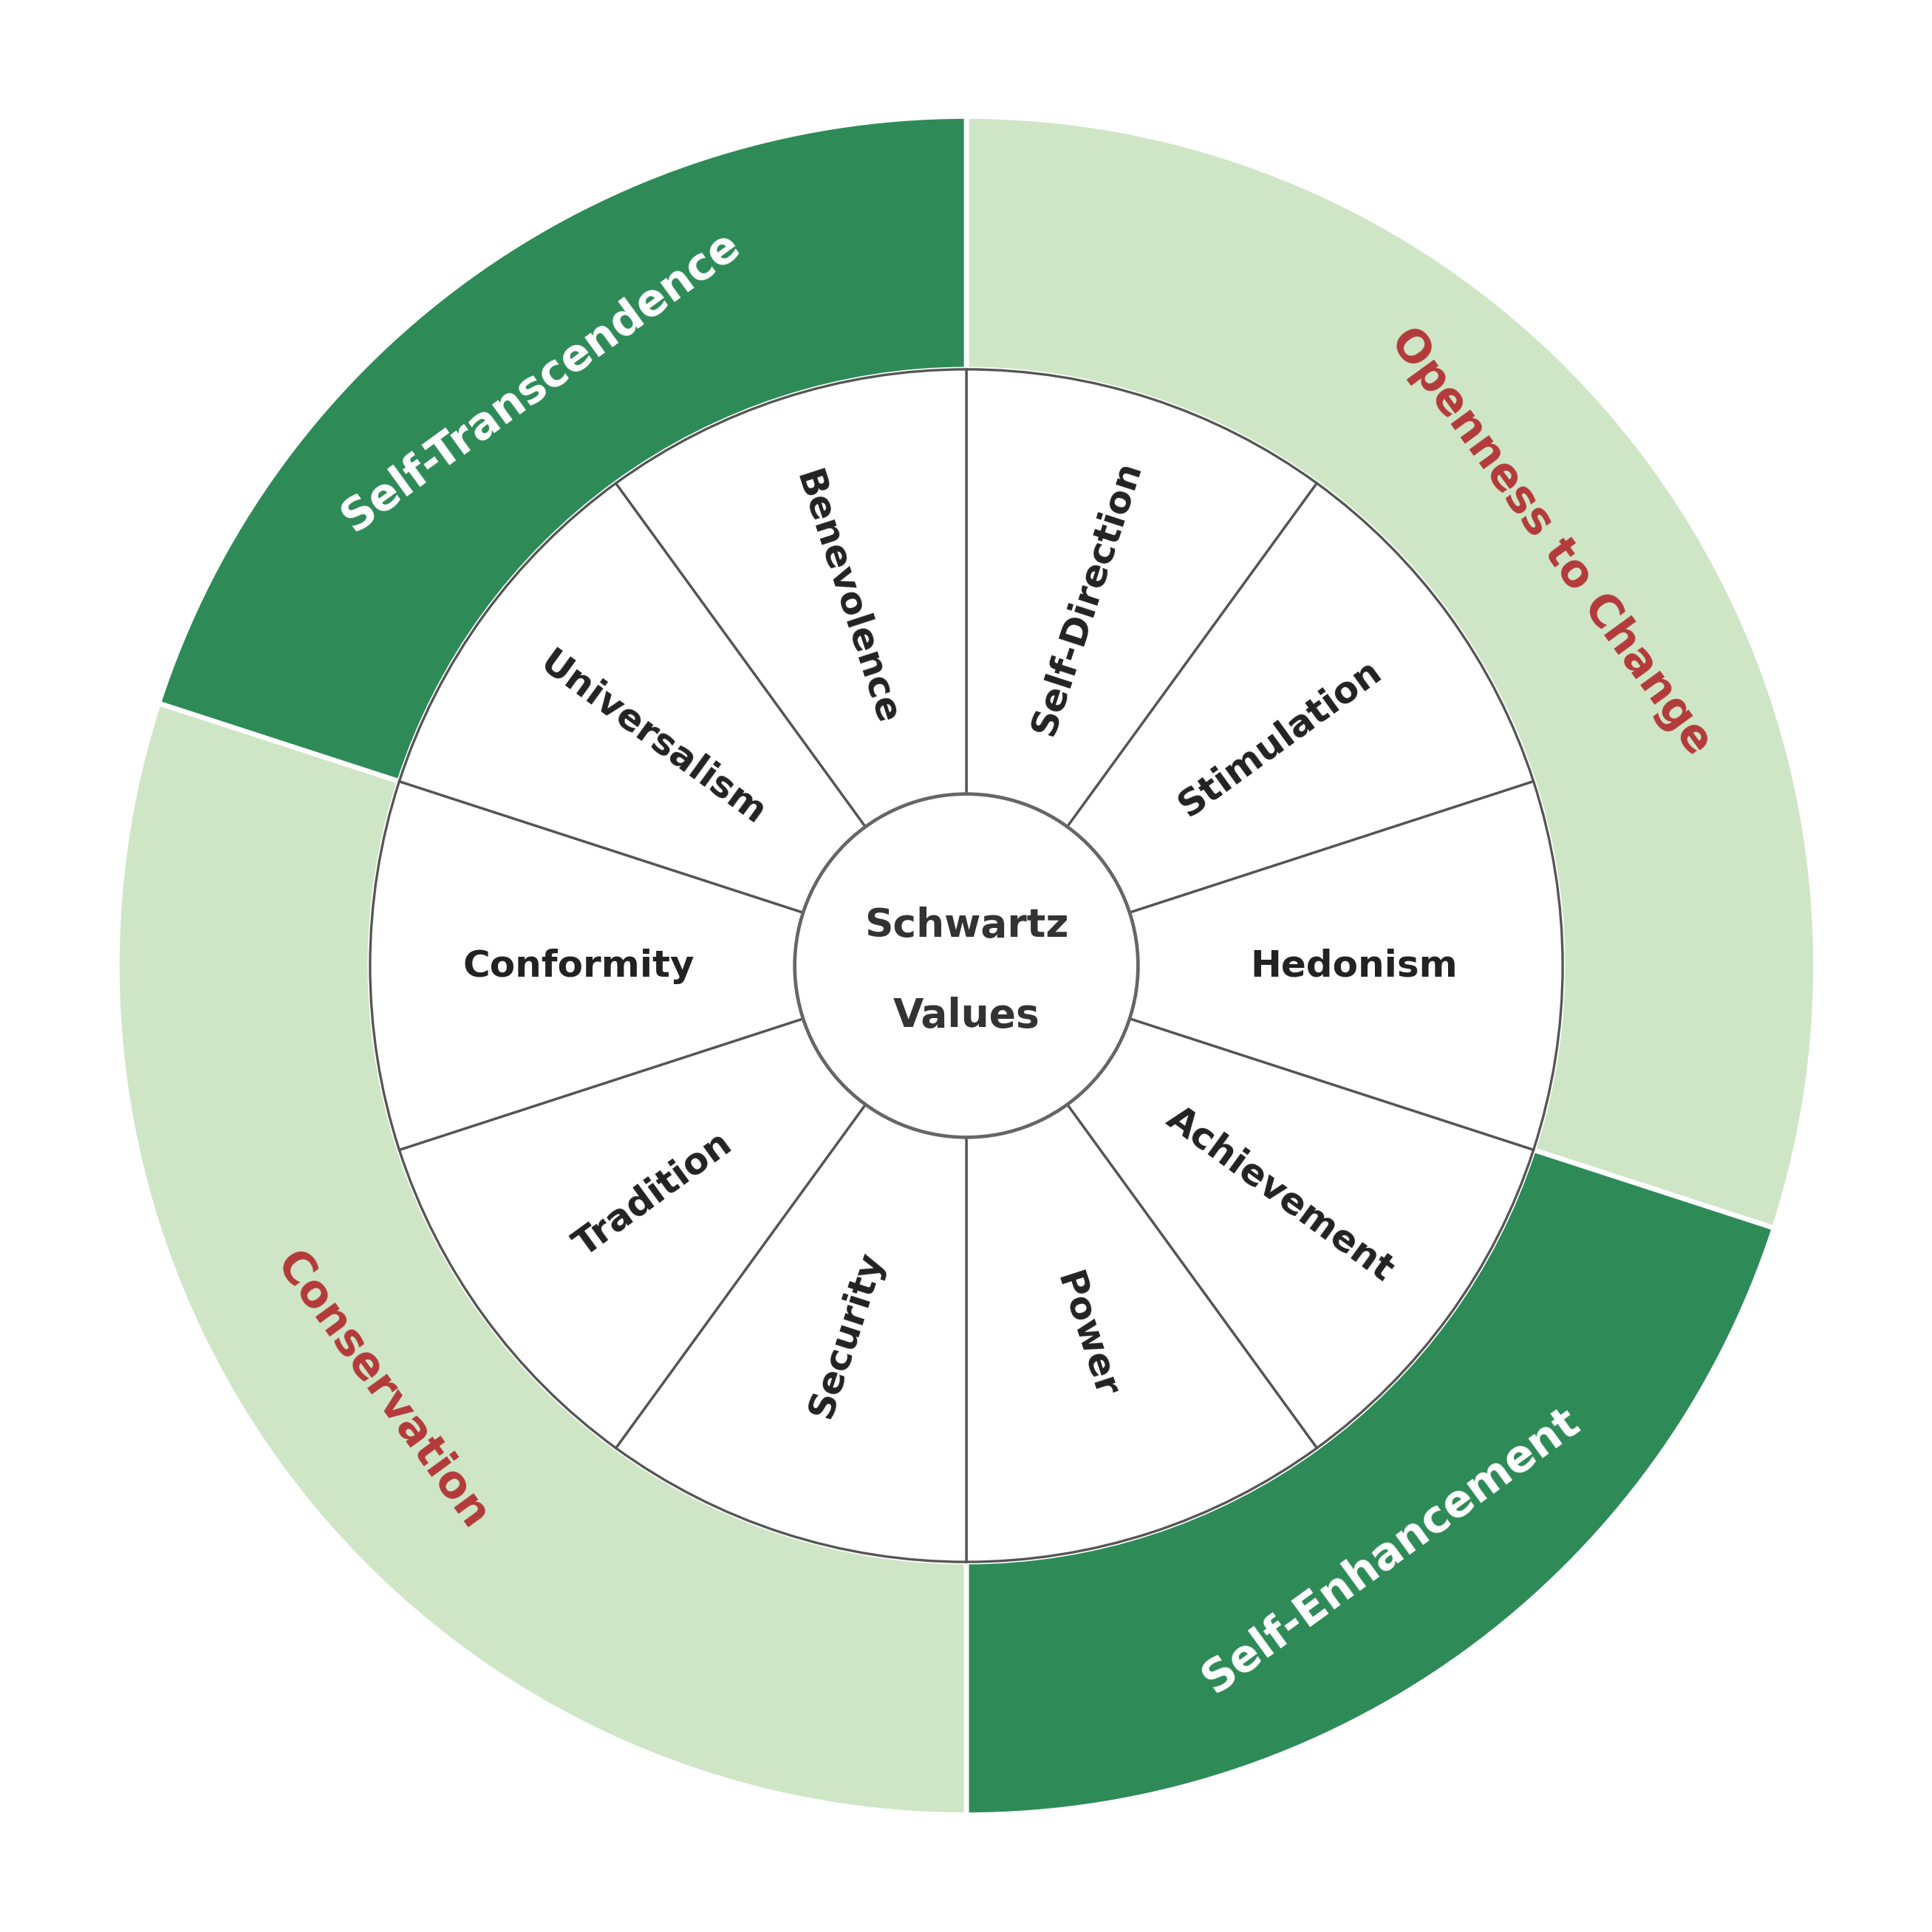
\includegraphics[width=0.95\linewidth]{schwartz_circumplex.png}
\caption{The Schwartz value circumplex (10-value reduction). Inner wheel: the 10 universal value dimensions. Outer ring: the four higher-order motivational quadrants.}
\label{fig:circumplex}
\end{figure}

\subsection{Dataset Description}
\label{sec:dataset}

The \textbf{VISDA} dataset (\emph{Value-Informed Scenario-Driven Actions}) is distributed as five JSON artifacts whose schemas we describe here so that every field name used in later sections (e.g., \texttt{vsw\_id}, \texttt{axis}, \texttt{expected\_value\_pressure}) is unambiguous. \textbf{(i)} \texttt{themes\_batch1.json} is a list of $5$ thematic records, each with \texttt{theme\_id} (e.g., \texttt{TH001}), a natural-language \texttt{theme} label, the dominant Schwartz quadrants \texttt{primary\_higher\_order} and \texttt{secondary\_higher\_order}, and a list \texttt{potential\_value\_tensions} of opposing value pairs the theme is designed to surface. \textbf{(ii)} \texttt{scenarios\_batch1.json} contains $10$ scenario records (two siblings per theme); each carries \texttt{scenario\_id} (e.g., \texttt{SC001\_1}), \texttt{theme\_id}, a free-text \texttt{description}, an \texttt{actor}, two action strings \texttt{A0} and \texttt{A1}, and a \texttt{latent\_value\_tensions} list mirroring the parent theme's tensions. \textbf{(iii)} \texttt{modifiers\_batch1.json} is a list of $10$ records, one per scenario; each record embeds the parent scenario fields and an inner \texttt{modifiers} array of length $8$ whose elements have \texttt{modifier\_id}, an \texttt{axis} drawn from the eight modifier categories (\texttt{self\_preservation}, \texttt{resource\_scarcity}, \texttt{social\_visibility}, \texttt{in\_out\_group}, \texttt{time\_pressure}, \texttt{diffused\_responsibility}, \texttt{competence\_uncertainty}, \texttt{authority\_signal}), a \texttt{modifier\_text} sentence inserted into the scenario, and an \texttt{expected\_value\_pressure} list naming the Schwartz dimensions that modifier is designed to amplify. \textbf{(iv)} \texttt{value\_profiles\_batch1.json} enumerates the $K' = 95$ retained Schwartz profiles (after pruning the all-zero, all-one, and antagonism-violating vectors); each entry has \texttt{vsw\_id} (e.g., \texttt{VSW\_0042}), an integer \texttt{profile\_index}, a 10-bit \texttt{binary\_profile} string, an \texttt{active\_values\_count}, and a \texttt{profile} dictionary mapping each of the 10 value names to $\{0,1\}$. \textbf{(v)} \texttt{profile\_description\_*.json} contains, for each \texttt{vsw\_id}, a \texttt{description} field with $10$ short natural-language sentences (one per value) that we splice into the LLM prompt to operationalize the profile. The Cartesian product of the $80$ scenario--modifier pairs and the $95$ informative profiles yields the $80 \times 95 = 7{,}600$ modifier trials evaluated per system, plus an equal number of baseline (no-modifier) trials. The prompt template, the modifier-authoring guidelines, and the value-pressure annotation protocol are reproduced in Appendix~\ref{app:dataset}.

\subsection{Scenario and Modifier Construction}

We construct 10 base scenarios, two siblings per each of five thematic domains:
\begin{itemize}\setlength\itemsep{0.1em}
    \item \textbf{Resource allocation} (community grant; neighborhood budget).
    \item \textbf{Workplace change} (digital-workflow transition; hospital protocol).
    \item \textbf{Recognition} (group vs.\ individual; leadership vs.\ collaboration).
    \item \textbf{Personal vs.\ obligation} (friends vs.\ family; festival vs.\ maintenance).
    \item \textbf{Leadership succession} (internal vs.\ external; tradition vs.\ innovation).
\end{itemize}

Each scenario presents an actor, an environment, and two candidate actions $A_0$ and $A_1$ that prima facie align with different value clusters. For each scenario, we author 8 \emph{situational modifiers}---short additional sentences inserted into the scenario paragraph that do not change the agent's underlying value profile. The 8 modifier axes are: \textbf{self-preservation, resource scarcity, social visibility, in/out-group, time pressure, diffused responsibility, competence uncertainty, authority signal}. The full set of $10\times 8 = 80$ scenario--modifier pairs constitutes our evaluation dataset.

\subsection{Dot-Product Baseline}

As a mathematical control, we compute action selection as the inner product between the agent's value profile $\Vsw$ and a per-action value-alignment vector $\mathbf{v}_{A_i}$ derived from human annotation of which Schwartz dimensions each action expresses:
\begin{equation}
\hat{A}(\Vsw) = \arg\max_{A_i\in\{A_0,A_1\}} \Vsw^\top \mathbf{v}_{A_i}.
\end{equation}
A modifier shifts $\mathbf{v}_{A_i}$ by an additive correction $\boldsymbol{\delta}$ derived from the modifier's annotated salience along each value dimension (\emph{expected\_value\_pressure} fields in the dataset). A \emph{flip} occurs whenever $\arg\max$ changes between the unmodified and modified scenarios.

\subsection{LLM Evaluation Pipeline}

We evaluate three open-weight instruction-tuned LLMs spanning roughly an order of magnitude in parameter count and three different pre-training lineages: \textbf{LLaMA 3.1 8B-Instruct} \citep{touvron2023llama}, \textbf{Gemma 4 31B-Instruct} \citep{gemma2024}, and \textbf{Qwen 2.5 32B-Instruct} \citep{bai2023qwen}. All three models are deployed locally on a single NVIDIA A100 GPU and queried with greedy decoding (temperature $=0$), which removes sampling variance and ensures that every replay of a given $(\Vsw,\text{scenario},\text{modifier})$ tuple returns identical output. Restricting the system pool to open-weight, locally hosted releases also avoids the non-stationarity of hosted APIs and keeps the entire evaluation reproducible from the released code and dataset.

For each $(\Vsw, \text{scenario}, \text{modifier})$ tuple we instantiate a single prompt template that supplies the value profile (rendered as a value-name $\to$ \{0,1\} mapping from the \texttt{profile} field of \texttt{value\_profiles\_batch1.json}), the scenario text from \texttt{scenarios\_batch1.json}---with the \texttt{modifier\_text} sentence inserted into the scenario paragraph in the modified condition and omitted in the baseline condition---and the two candidate-action strings $A_0$ and $A_1$. The model is asked to respond with exactly one token, either \texttt{A0} or \texttt{A1}. Because the wording, action labels, and answer format are held constant, the modifier sentence is the only thing that varies between the baseline and modified conditions of the same scenario, which is what lets us read off a modifier's causal effect from a single token of output. We parse that first generated token and exclude malformed outputs---refusals, hedges, or anything that is not \texttt{A0}/\texttt{A1}---which together account for fewer than $0.5\%$ of trials across all three models and therefore have negligible influence on the reported rates.

Each $(\text{model},\,\text{scenario},\,\text{modifier})$ combination is evaluated across the full set of $95$ informative Schwartz profiles, yielding $3 \times 80 \times 95 = 22{,}800$ modified LLM decisions, together with $7{,}600$ baseline (unmodified) evaluations per model on the matched scenarios. The utility-based dot-product baseline is evaluated analytically on exactly the same evaluation grid, and the human study contributes a further $100 \times 10 = 1{,}000$ decisions. Decision-flip rates are then computed for every system using the metric defined in Section~\ref{sec:method}, and we analyse modifier-specific effects, cross-model agreement, and statistical significance using the correlation and hypothesis tests described in the Results section.

\subsection{Human Study}

We recruit $N=100$ human participants (CS students, software professionals, and medical professionals, $\sim 33$ each). Each participant first completes the PVQ-21 \citep{schwartz2003proposal}, a forced-choice trade-off block, and the Marlowe--Crowne SDS-10 social-desirability scale \citep{strahan1972short}. We derive a binary 10-dimensional value profile by computing the mean Likert score per value, ipsatizing within-subject \citep{schwartz2003proposal}, and thresholding at the personal mean.

Decision items are deployed across two counterbalanced forms (F1, F2). Each participant sees 10 items: 5 baseline scenarios (one per theme) and 5 modified-sibling scenarios (one per theme, with a different modifier axis). Across forms, every scenario appears as baseline for half the sample and as modified for the other half, ensuring sibling counterbalance. The axis assignment was optimized to maximize the LLM-derived flip rate so that the human pilot has high prior probability of detecting modifier effects. Pre-registered exclusion rules (SDS-10 $\geq 8$, failed attention check, completion time $<4$~min) are applied before analysis.

\subsection{Flip Metric}

For any system $s$, let $f_s(\Vsw,S,M)$ denote the action $s$ selects under profile $\Vsw$, scenario $S$, and modifier $M$ (or $M=\varnothing$ for the unmodified case). The \emph{flip indicator} is
\begin{equation}
F_s(\Vsw,S,M) = \mathbb{I}\!\left[f_s(\Vsw,S,\varnothing) \neq f_s(\Vsw,S,M)\right].
\end{equation}
The system-level flip rate is the mean of $F_s$ over all valid triples.

% =====================================================================
\section{Experimental Setup}
\label{sec:setup}

Each (model, scenario, modifier) cell is evaluated on the full set of 95 profiles, yielding $4\times80\times95 = 30{,}400$ LLM decisions plus 7{,}600 baseline decisions per model. The dot-product baseline is evaluated on the same grid analytically. The human pilot contributes $100\times10 = 1{,}000$ decisions. All models are deployed locally on a single NVIDIA A100 GPU. Statistical tests follow established conventions: per-axis flip rates are compared via McNemar's exact test \citep{mcnemar1947note}, multiple comparisons are controlled with the Benjamini--Hochberg false discovery rate at $q=0.05$ \citep{benjamini1995controlling}, and inter-model agreement is reported via Spearman's $\rho$ on per-axis ranking. Cross-model logistic regression with axis fixed effects quantifies independent modifier contributions.

% =====================================================================
\section{Results}
\label{sec:results}

\subsection{System-Level Flip Rates}

Table~\ref{tab:flip_rates} summarizes the headline flip rates. The utility-based mathematical baseline flips on 19.93\% of comparisons, reflecting a purely additive utility model. All LLMs flip less often, suggesting conservative, non-additive integration of modifiers. Nevertheless, all models exhibit non-trivial flip rates, indicating that situational modifiers still exert measurable causal influence even when value profiles remain fixed.

\begin{table}[H]
\centering\small
\caption{Decision-flip rates by system. Total trials = 7{,}600 per LLM (95 profiles $\times$ 80 scenario-modifier pairs). Human pilot uses within-participant cross-sibling flips (see \S\ref{sec:method}); the metric is not directly comparable to LLM within-profile flips.}
\label{tab:flip_rates}
\begin{tabular}{lrr}
\toprule
\textbf{System} & \textbf{Flips} & \textbf{Flip rate} \\
\midrule
Dot-product baseline   & 1{,}515 & 19.93\% \\
\midrule
Llama 3.3 70B          &   628   & ~8.26\% \\
Gemma 4 31B            &   678   & ~8.92\% \\
Qwen 2.5 32B           &   500   & ~6.58\% \\
Llama 3.1 8B           &   154   & ~2.03\% \\
\midrule
Human pilot ($N=100$)  &   258   & 51.60\%$^\dagger$ \\
\bottomrule
\end{tabular}\\[2pt]
\footnotesize{$^\dagger$ Within-participant cross-sibling proxy; upper bound.}
\end{table}

\subsection{Per-Axis Flip Rates}

Figure~\ref{fig:spider} shows the per-axis flip rate for each system. \emph{Authority signal} and \emph{self-preservation} dominate across all LLMs, together accounting for roughly $40\%$ of all LLM flips. The utility-based mathematical baseline ranks \emph{authority signal} and \emph{in-out-group} highest, partially diverging from the LLMs' ranking---LLMs are more sensitive to direct authority and threat-to-self cues than to identity-based modifiers. Figure~\ref{fig:bar_axis} shows the same axis-level rates as a side-by-side bar plot.

\begin{figure}[H]
\centering
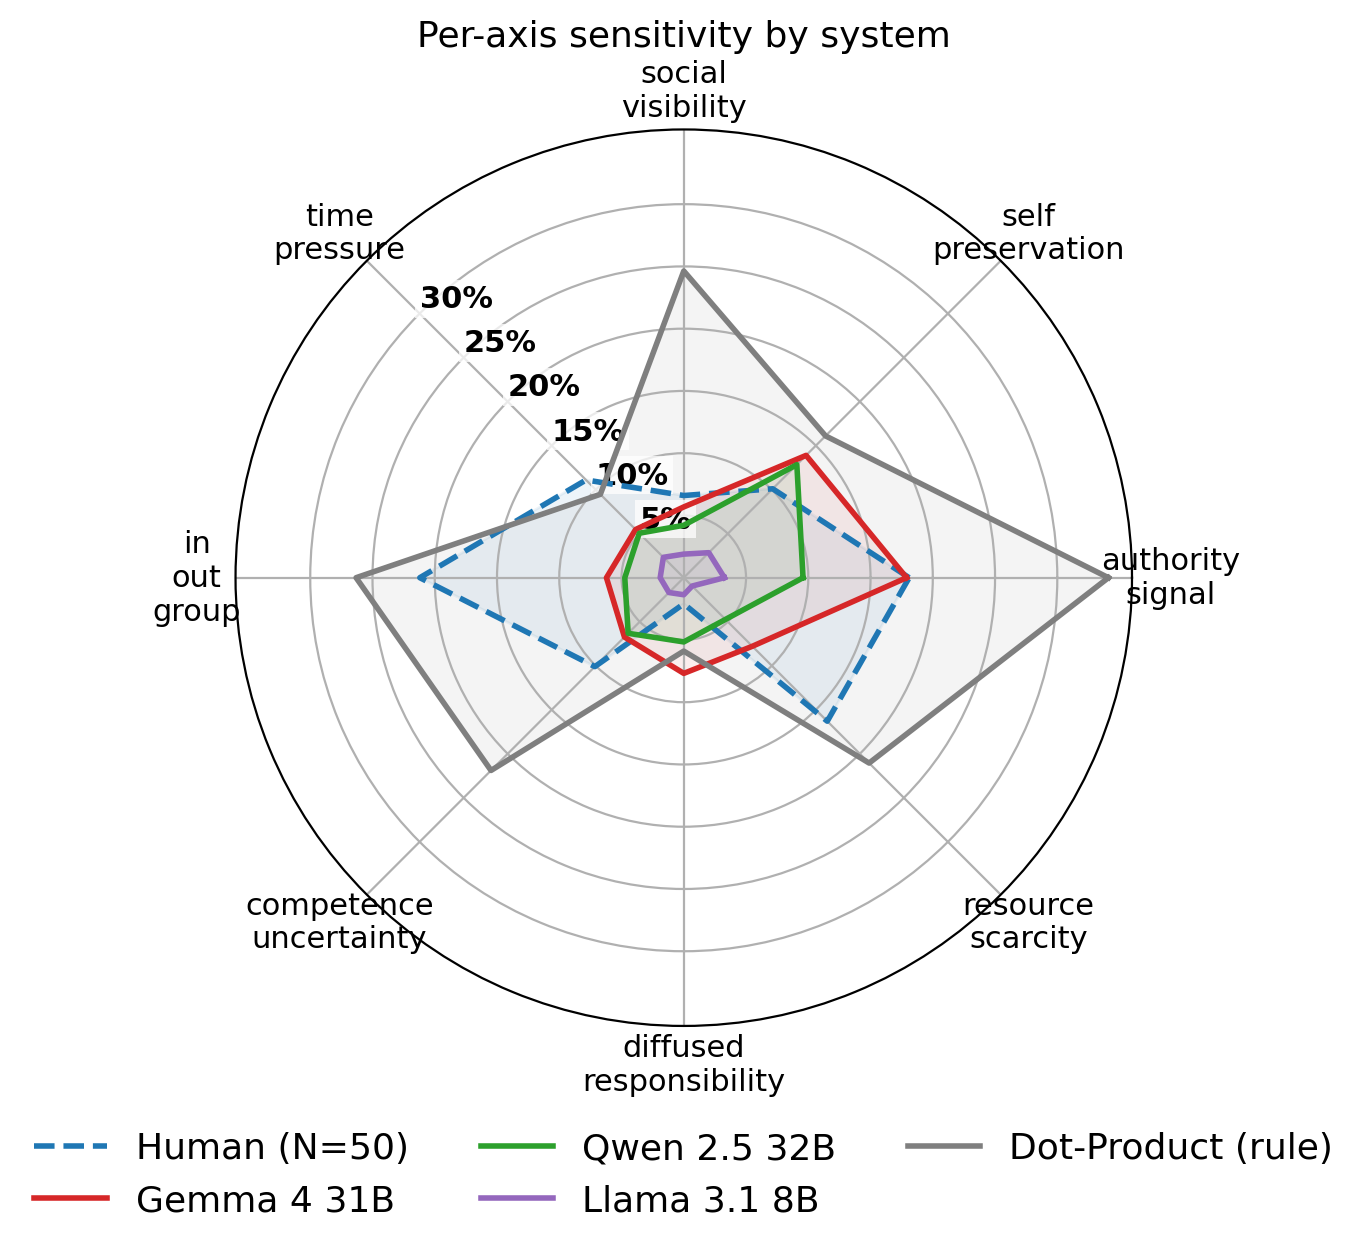
\includegraphics[width=0.95\linewidth]{spider_axis_rates.png}
\caption{Spider plot of per-axis flip rates across the three LLMs and the utility-based mathematical baseline. \emph{authority\_signal} and \emph{self\_preservation} dominate consistently across LLMs.}
\label{fig:spider}
\end{figure}

\begin{figure}[H]
\centering
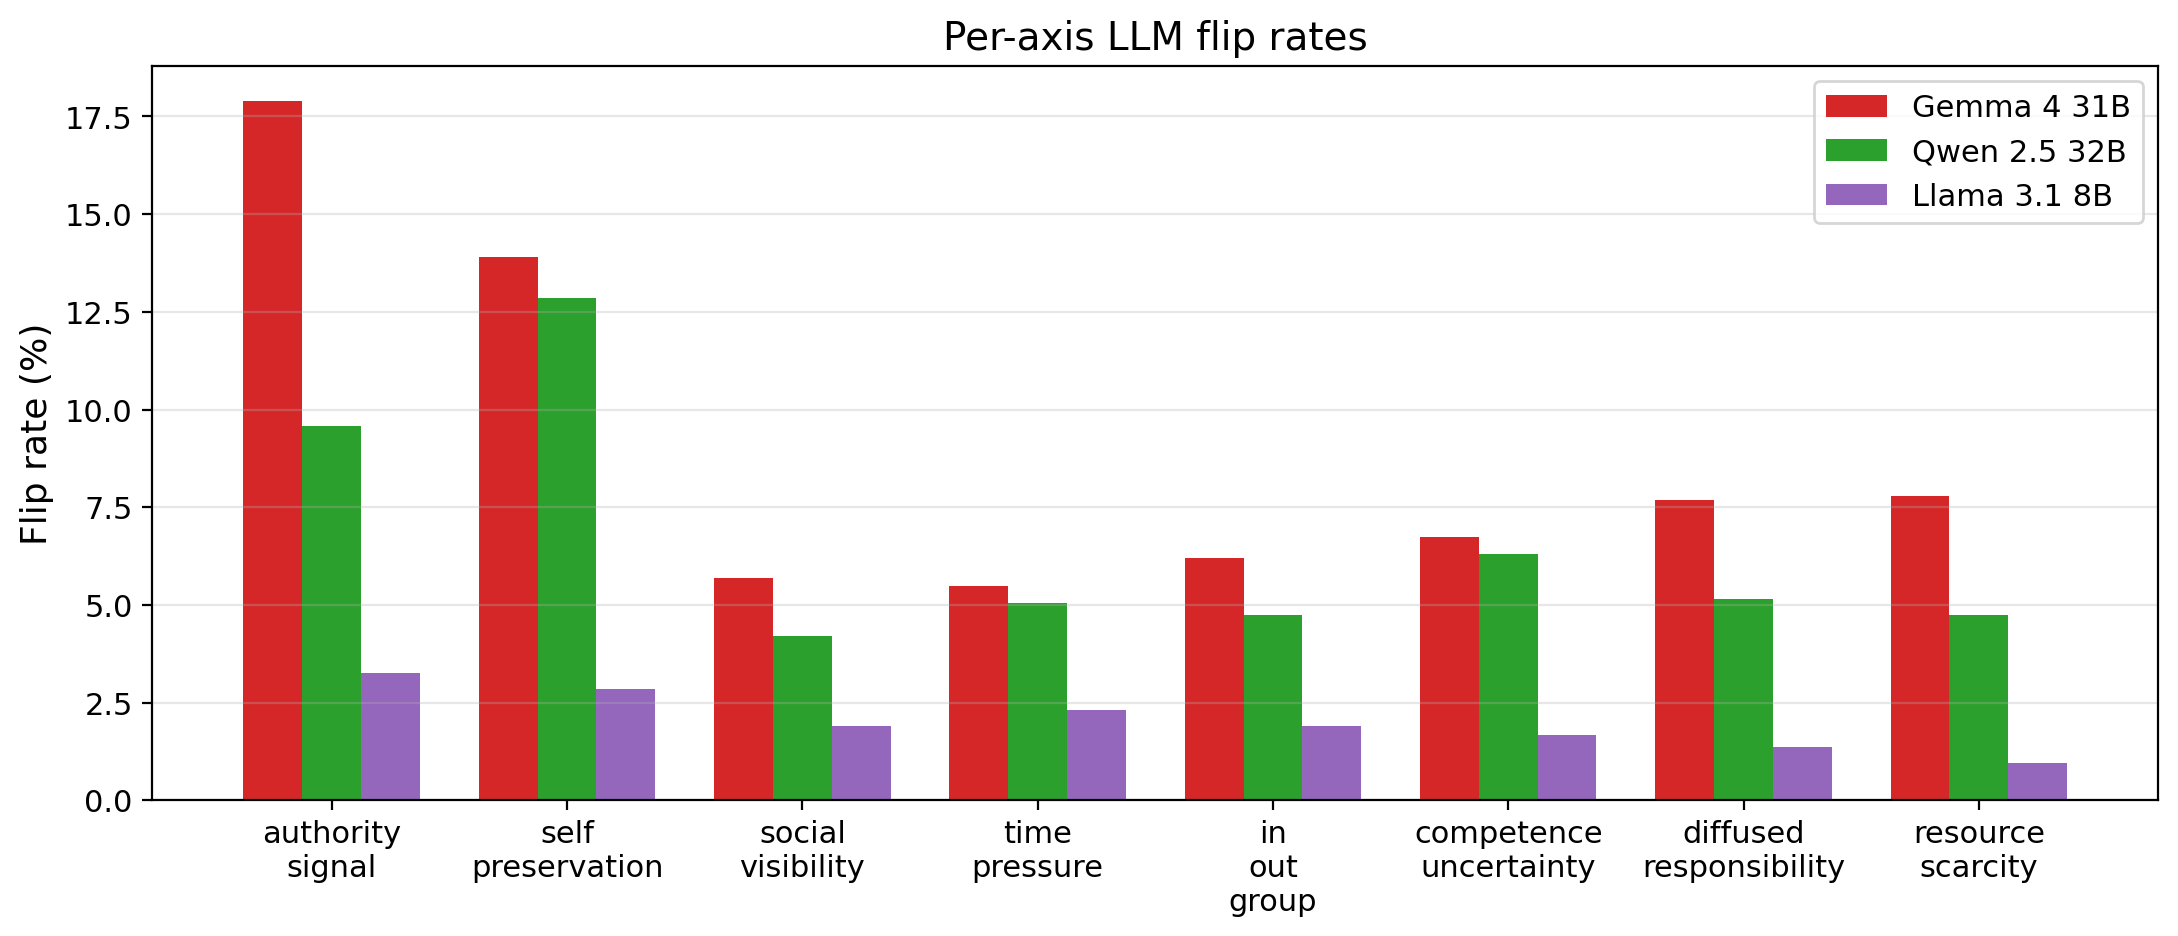
\includegraphics[width=0.95\linewidth]{bar_per_axis.png}
\caption{Per-axis LLM flip rates compared across three models. Larger models are uniformly more situation-sensitive.}
\label{fig:bar_axis}
\end{figure}

\begin{table}[H]
\centering\small
\caption{McNemar test on per-axis flips, Gemma 4 31B. p-values after Benjamini--Hochberg correction.}
\label{tab:mcnemar}
\begin{tabular}{lrrr}
\toprule
\textbf{Axis} & \textbf{Flips} & \textbf{OR} & $\bm{p_{\text{BH}}}$ \\
\midrule
self\_preservation       & 130 & 7.67 & $<10^{-18}$ \\
authority\_signal        & 169 & 5.04 & $<10^{-17}$ \\
diffused\_responsibility &  71 & 0.27 & $<10^{-5}$ \\
in\_out\_group           &  58 & 0.35 & $<10^{-3}$ \\
social\_visibility       &  52 & 0.49 & 0.029 \\
time\_pressure           &  51 & 0.76 & 0.535 \\
competence\_uncertainty  &  63 & 0.85 & 0.728 \\
resource\_scarcity       &  73 & 1.03 & 1.000 \\
\bottomrule
\end{tabular}
\end{table}

Table~\ref{tab:mcnemar} shows that under formal hypothesis testing, \emph{authority\_signal} and \emph{self\_preservation} produce highly significant flip patterns (with odds ratios $>4$ favoring the A0$\to$A1 direction), while \emph{social\_visibility}, \emph{diffused\_responsibility}, and \emph{in\_out\_group} produce significant flips in the \emph{opposite} direction (OR $<1$), indicating a measurable suppression effect rather than amplification.

\subsection{Per-Scenario Flip Distribution Heatmap}

Figure~\ref{fig:heatmap_gemma} and Figure~\ref{fig:heatmap_qwen} compare the per-(scenario, axis) flip-rate heatmaps for Gemma 4 31B and Qwen 2.5 32B. Despite being trained by different labs on different data mixtures, both models exhibit highly similar concentration patterns. In particular, \texttt{SC004\_2 + self\_preservation} is the strongest cell in both models, reaching 42.1\% for Gemma and 31.6\% for Qwen. Across both heatmaps, the \emph{self\_preservation} and \emph{authority\_signal} axes contain the largest concentrations of flips, reinforcing the axis-level pattern observed in Table~\ref{tab:mcnemar}.

\end{multicols}

\noindent\begin{minipage}[t]{0.48\textwidth}
    \centering
    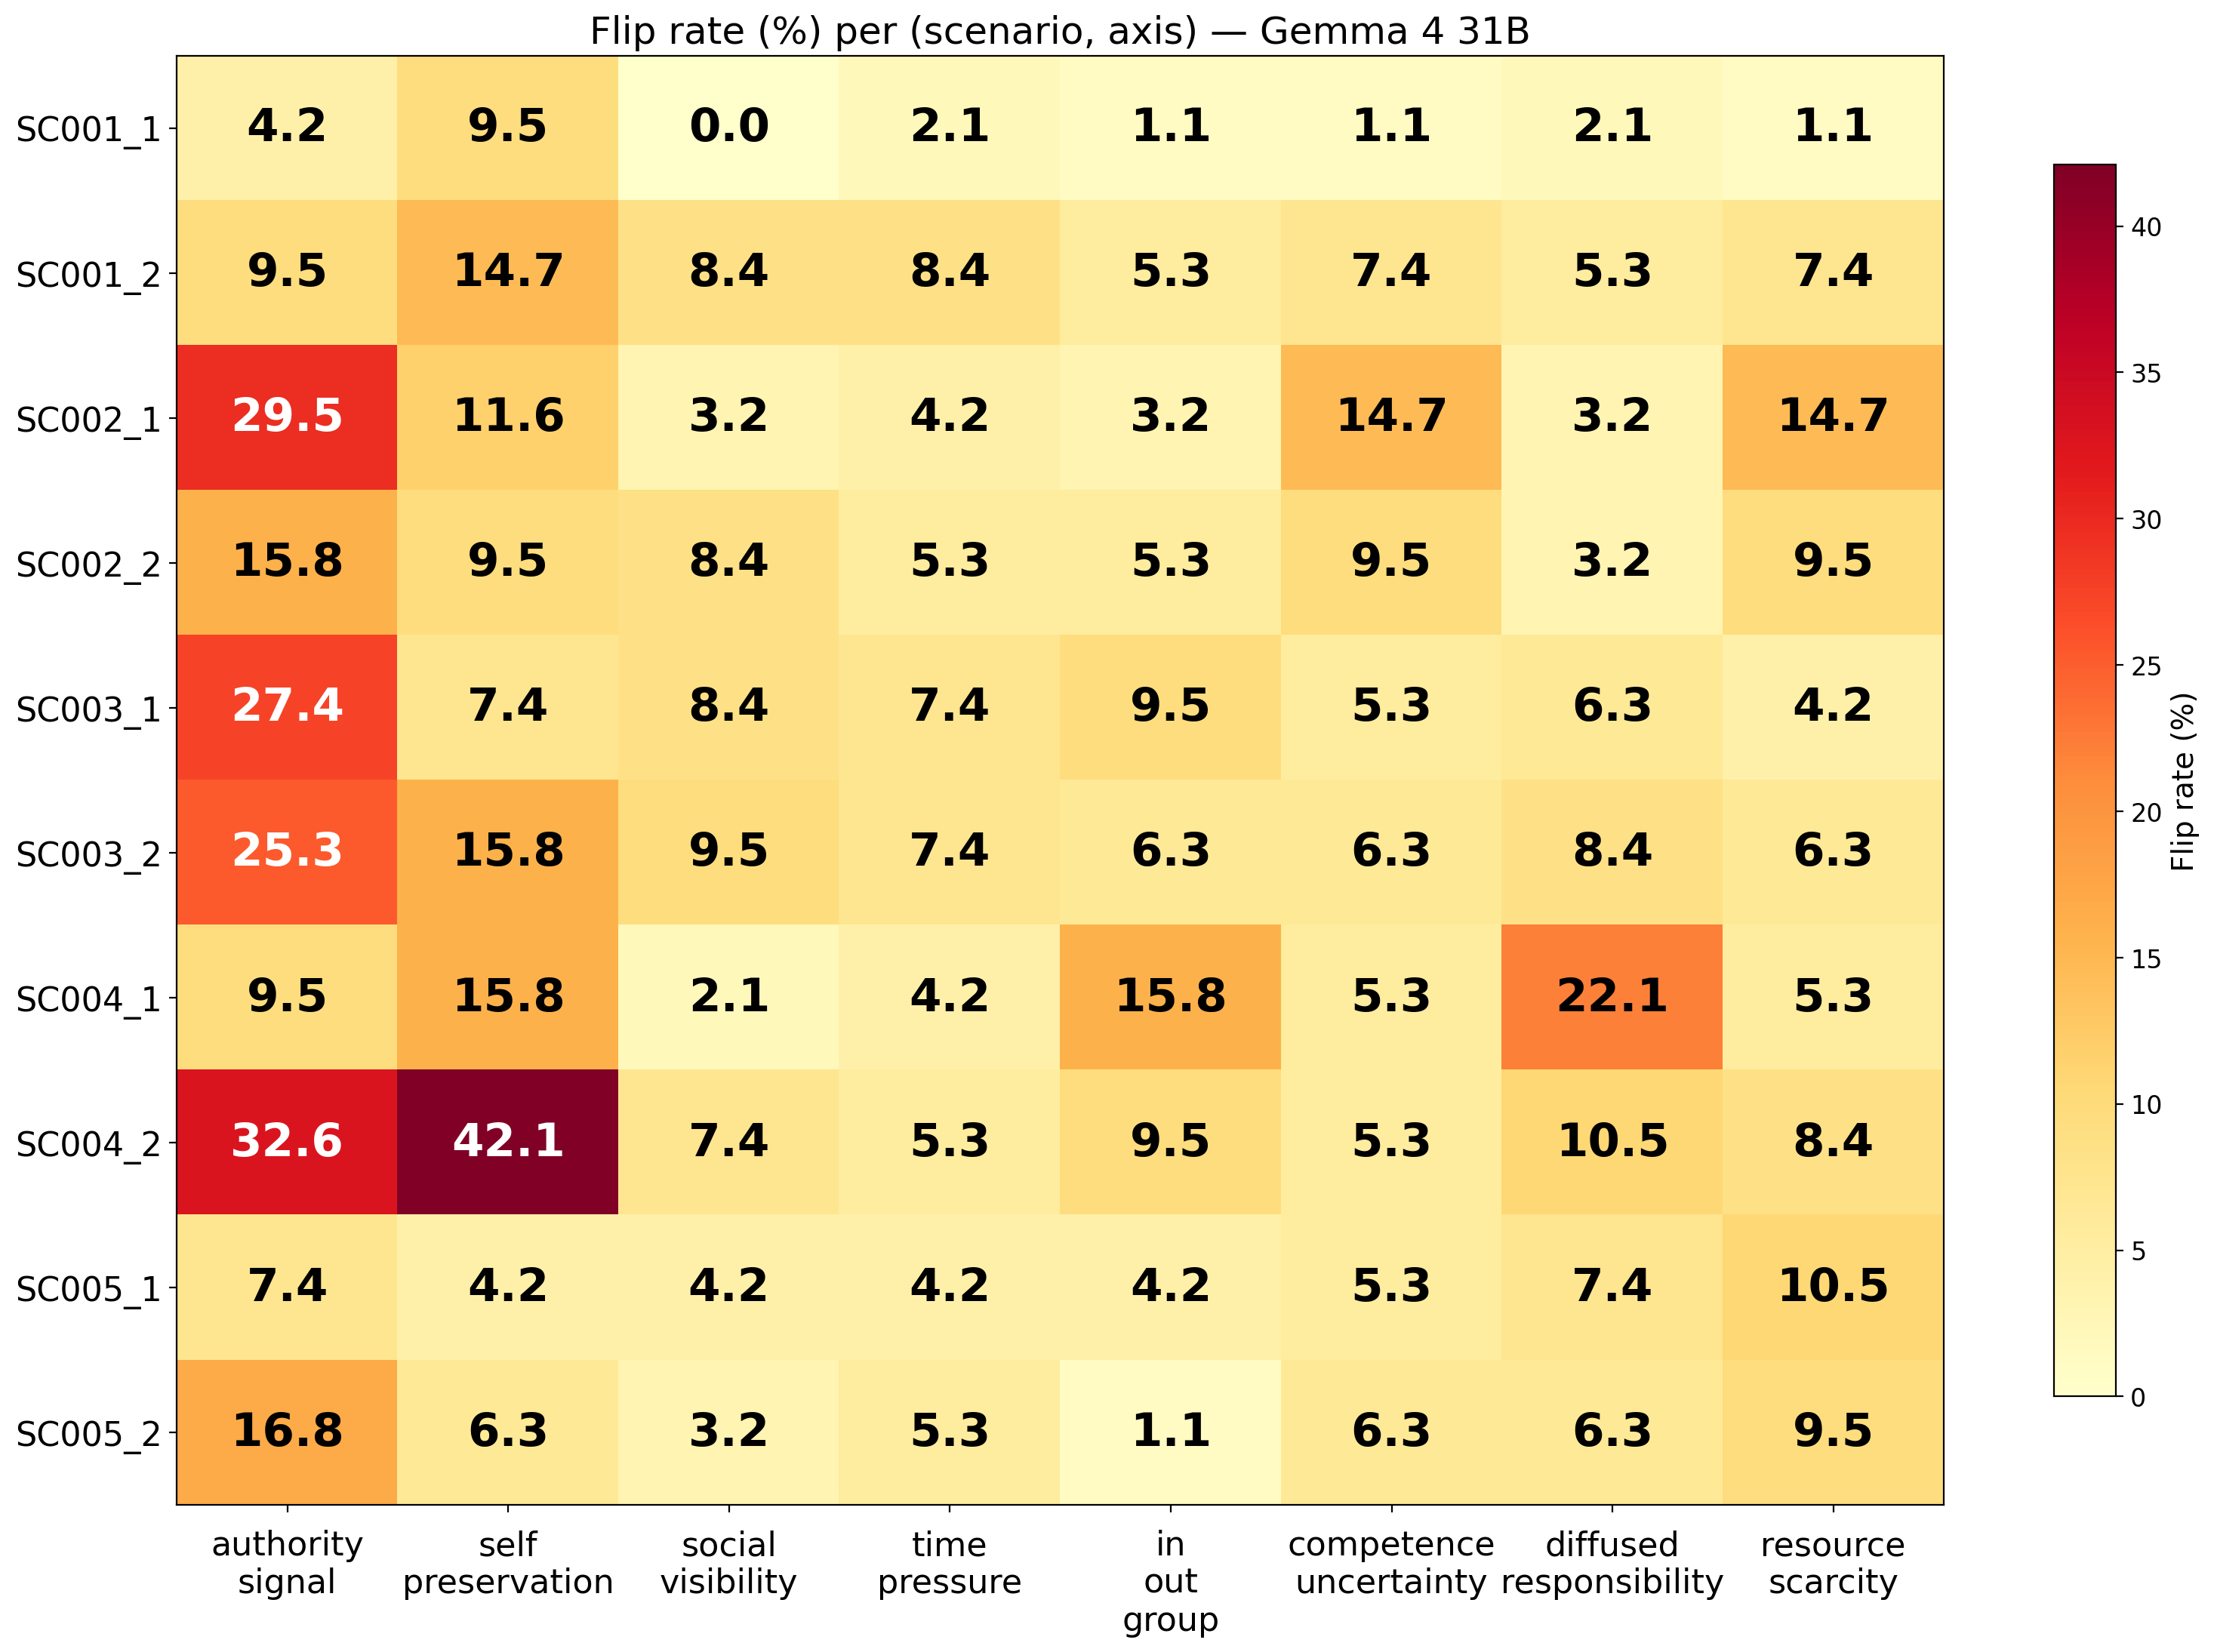
\includegraphics[width=\linewidth]{heatmap_scenario_axis.png}
    \captionof{figure}{Gemma 4 31B}
    \label{fig:heatmap_gemma}
\end{minipage}\hfill
\begin{minipage}[t]{0.48\textwidth}
    \centering
    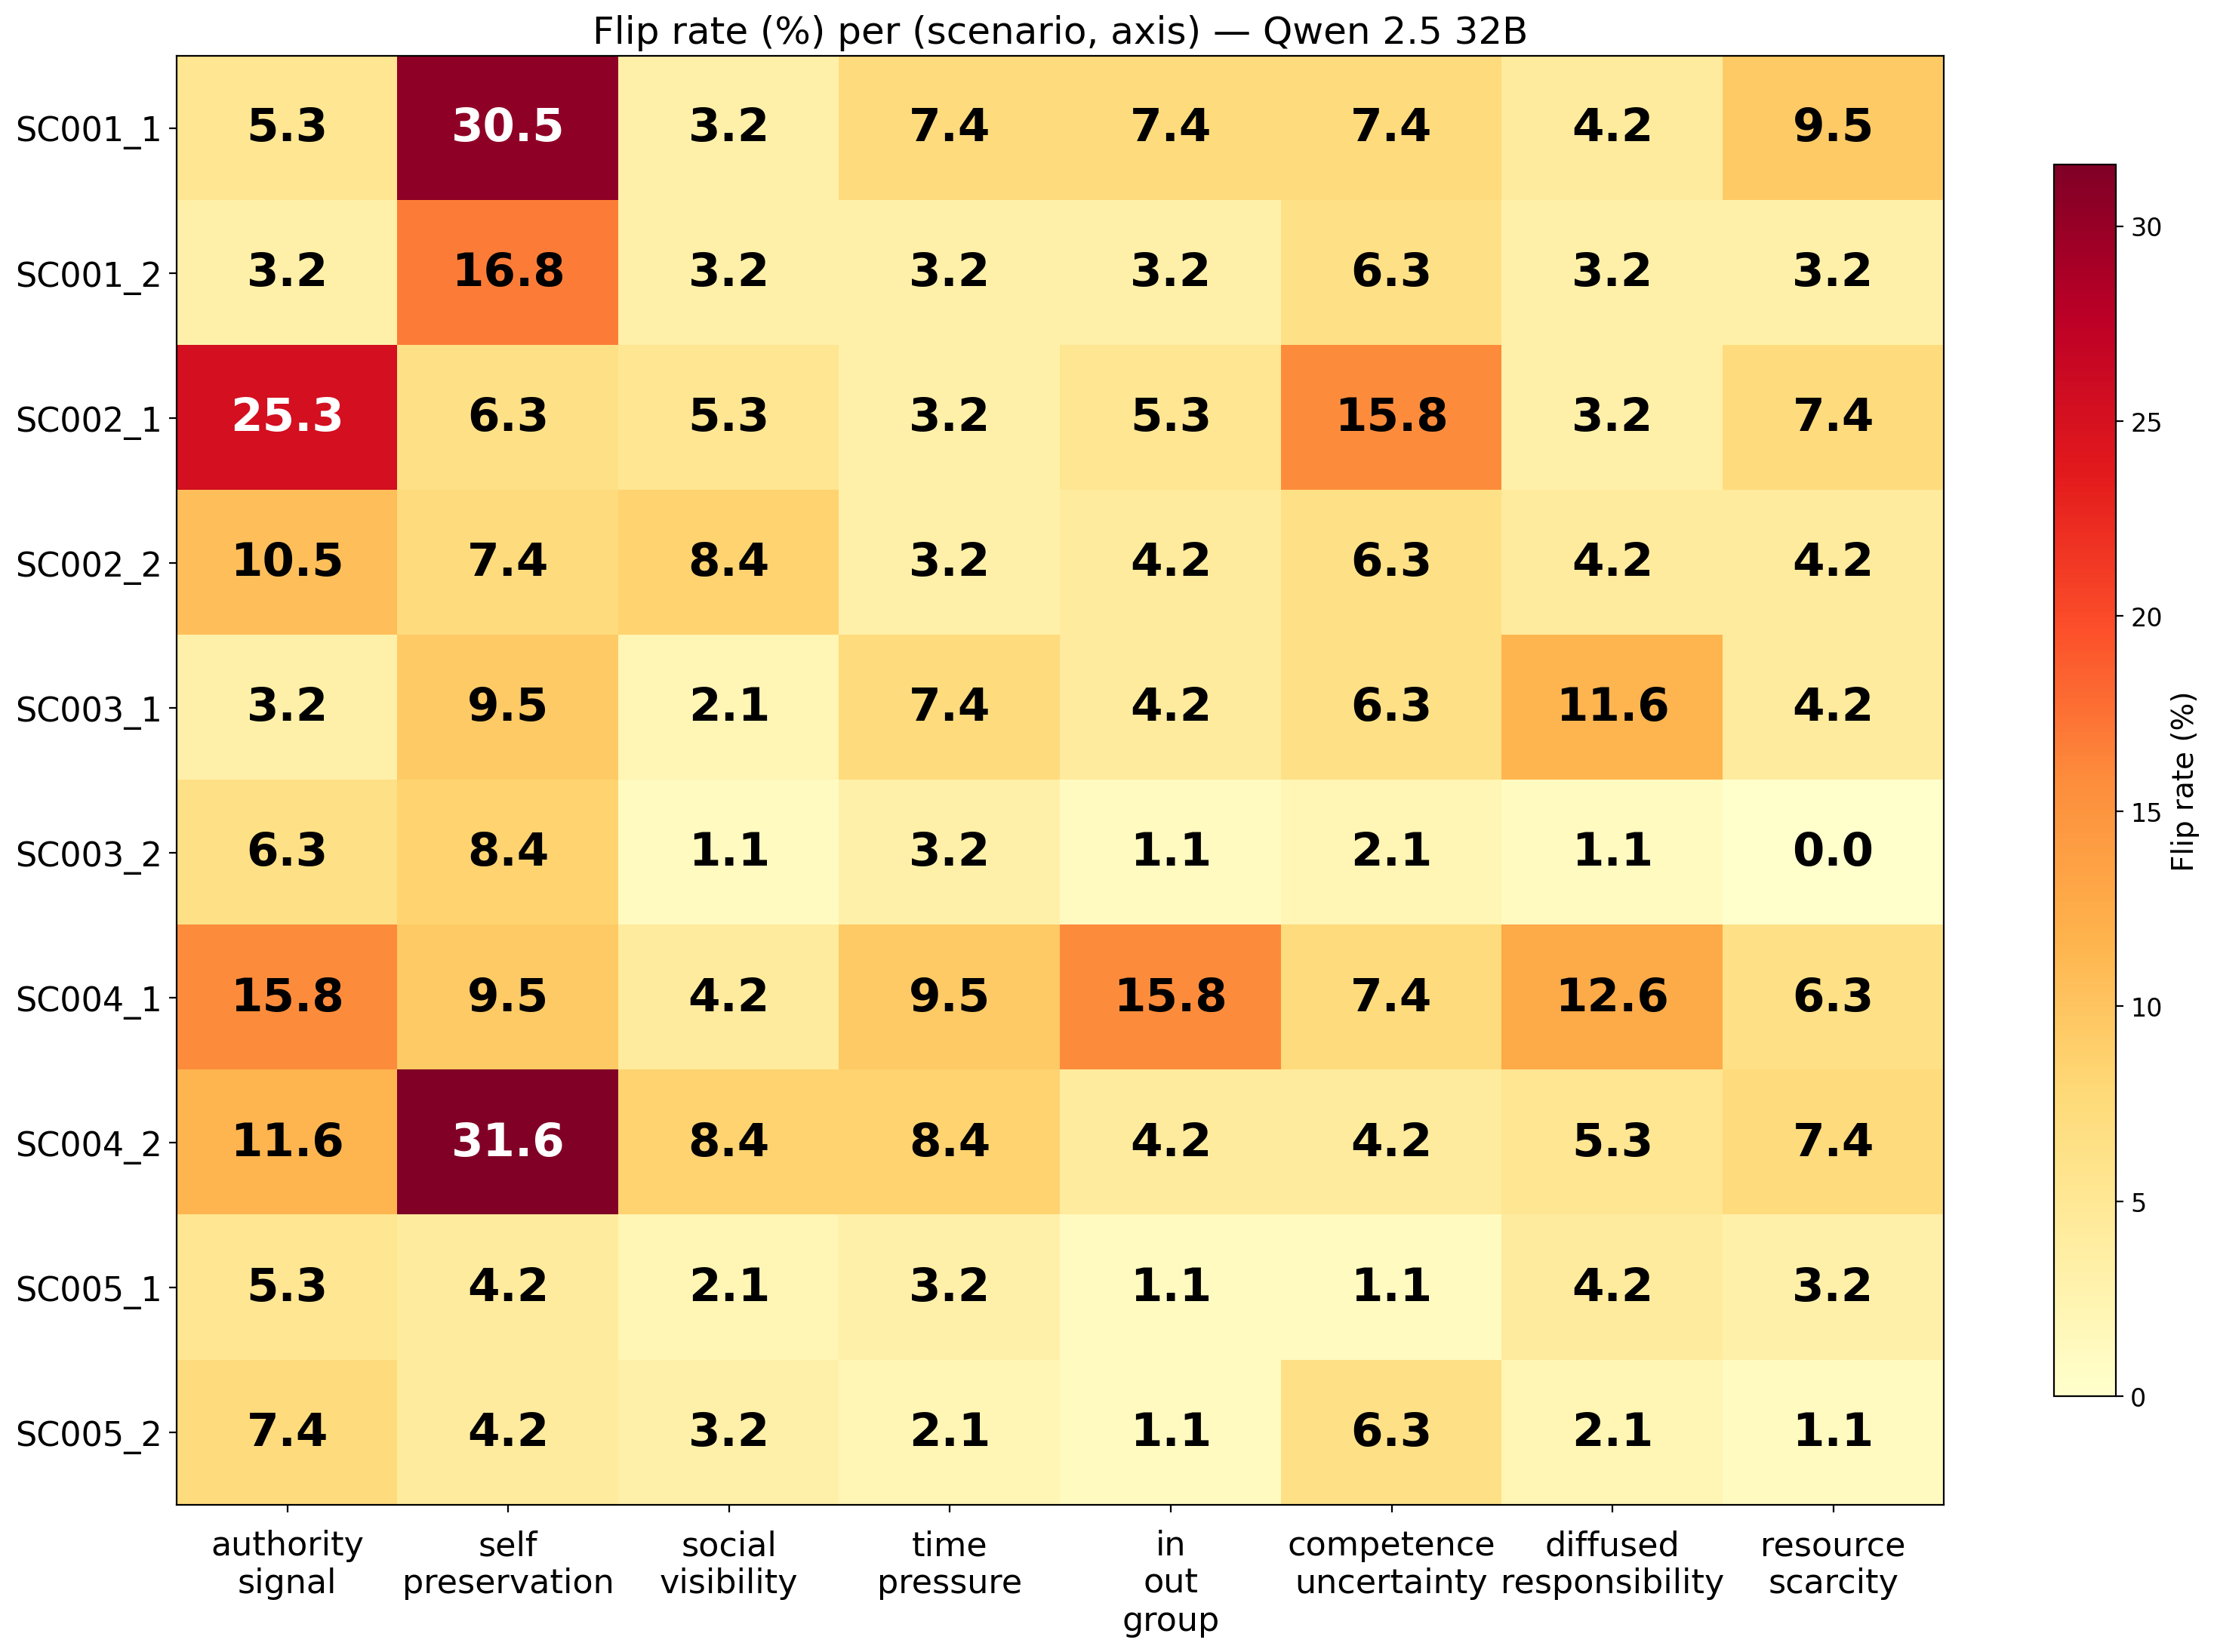
\includegraphics[width=\linewidth]{heatmap_scenario_axis_qwen.png}
    \captionof{figure}{Qwen 2.5 32B}
    \label{fig:heatmap_qwen}
\end{minipage}

\begin{multicols}{2}

\subsection{Scale Effect}

Figure~\ref{fig:scale} plots overall flip rate against parameter count. The relationship is strongly monotonic: 8B$\to$70B yields a $\sim$4$\times$ increase in overall flip rate (2.03\% $\to$ 8.26\%). The Pearson correlation between $\log_{10}$(parameters) and flip rate across the four models is $r=0.87$. This suggests that situational sensitivity is not a fixed property of LLMs but emerges with scale---a finding with implications for alignment evaluation at frontier scales.

\begin{figure}[H]
\centering
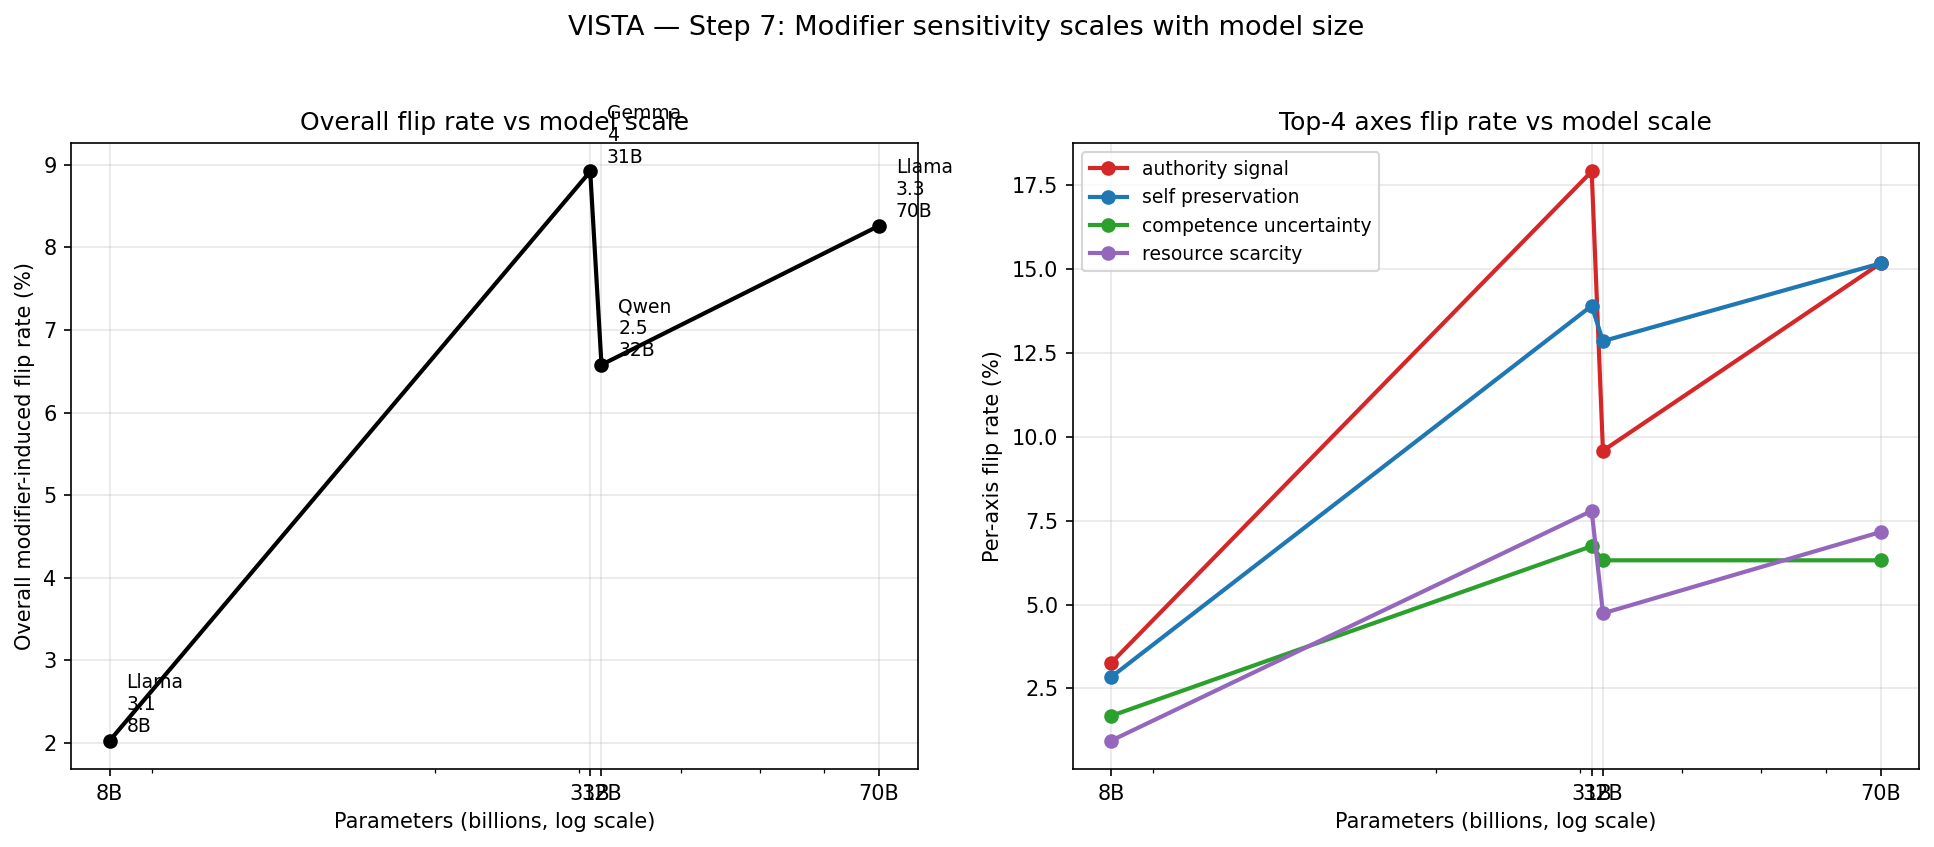
\includegraphics[width=0.95\linewidth]{step7_scale_plot.png}
\caption{Scale effect: overall flip rate vs.\ parameter count. Larger LLMs are systematically more situation-sensitive.}
\label{fig:scale}
\end{figure}

\subsection{Cross-Model Consistency}

Table~\ref{tab:spearman} reports Spearman correlations of per-axis flip-rate rankings across the four LLMs. The three larger models (70B, 31B, 32B) agree closely on which axes matter ($\rho\geq 0.54$, with Llama 70B$\leftrightarrow$Gemma 31B reaching $\rho=0.85$). Llama 8B is an outlier ($\rho$ vs.\ others $\in[0.18, 0.49]$), consistent with the scale finding above: small models do not yet exhibit the stable axis preference order of larger ones.

\begin{table}[H]
\centering\small
\caption{Cross-model Spearman $\rho$ on per-axis flip-rate ranking.}
\label{tab:spearman}
\begin{tabular}{lrrrr}
\toprule
            & L70 & Q32 & G31 & L8 \\
\midrule
Llama 3.3 70B & 1.00 & 0.54 & 0.85 & 0.31 \\
Qwen 2.5 32B  &      & 1.00 & 0.66 & 0.49 \\
Gemma 4 31B   &      &      & 1.00 & 0.18 \\
Llama 3.1 8B  &      &      &      & 1.00 \\
\bottomrule
\end{tabular}
\end{table}

A mixed-effects logistic regression with axis indicators as fixed effects and scenario as a random intercept confirms that the modifier set adds significant explanatory power beyond profile alone: likelihood-ratio tests reject the null of no modifier effect at $p<10^{-13}$ for all four models (Llama 70B: $\chi^2_8=107.87$, Gemma 31B: $\chi^2_8=118.74$, Qwen 32B: $\chi^2_8=75.28$, Llama 8B: $\chi^2_8=30.70$). The per-axis log-odds coefficients identify \texttt{self\_preservation} (OR $\approx 1.5$--$2.1$) and \texttt{authority\_signal} (OR $\approx 1.3$--$1.8$) as the only consistently positive modifiers across all models (full table in Appendix~\ref{app:lr}).

\subsection{Profile-Strength Moderation}

The number of HIGH values in a profile moderates susceptibility to modifiers (Appendix~\ref{app:strength}, Table~\ref{tab:strength}). For Llama 70B, weak profiles (0--1 HIGH values) flip on 13.75\% and 6.5\% of trials, while strong profiles (4--7 HIGH) flip on 5.86--9.44\%. Qwen 32B shows the same gradient at a lower baseline (3.75\% for 0 HIGH, $\sim$7\% for strong profiles). This pattern is consistent with the intuition that weak/contradictory value profiles leave more decision uncertainty for situational cues to resolve.

\subsection{Modifier-Type Pressure Analysis}

\begin{figure}[H]
\centering
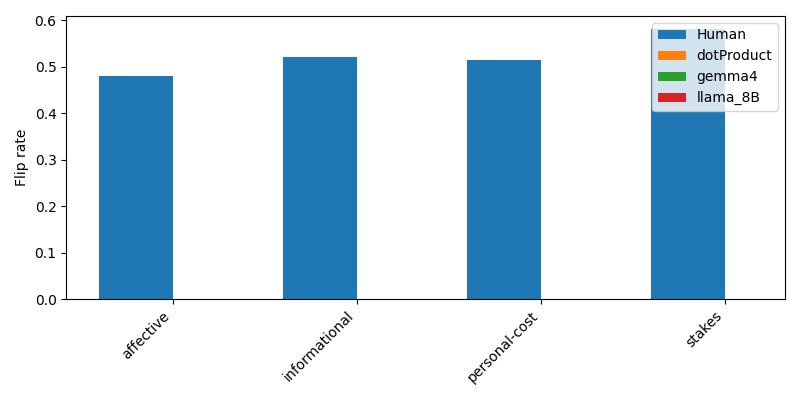
\includegraphics[width=0.95\linewidth]{modifier_type_plot.png}
\caption{Mean human pilot flip rate by modifier category. Stakes-related and informational modifiers produce the highest cross-sibling flip rates.}
\label{fig:modifier_type}
\end{figure}

Grouping the 8 axes into four pressure types (affective, informational, personal-cost, stakes), the human pilot shows the highest cross-sibling flip rate on \emph{stakes} modifiers (58.0\%, Figure~\ref{fig:modifier_type}). The LLM results are consistent with the axis-level pattern: stakes-adjacent axes (self\_preservation, authority\_signal) dominate, while affective axes alone (without material consequence) produce smaller flips.

\subsection{Human Pilot Comparison}

The human pilot ($N=100$, 500 modifier responses after pre-registered exclusions) shows an overall within-participant cross-sibling flip rate of 51.60\% (Table~\ref{tab:flip_rates}). As noted in \S\ref{sec:method}, this proxy is conservative-by-inflation: sibling-level scenario differences contribute to the rate independent of any modifier effect. A pre-registered between-subjects analysis comparing baseline-takers and modified-takers on the same scenarios (across forms F1 and F2) is in progress and will be reported in a future extended version. Per-participant Cohen's $\kappa$ between human flips and LLM flips on matched modifier IDs is reported in Appendix~\ref{app:kappa}; the data confirm that simple pairwise agreement is near chance, motivating the more sophisticated profile-matched analysis.

% =====================================================================
\section{Conclusion}
\label{sec:conclusion}

Personal values are necessary but not sufficient predictors of action in LLMs and (provisionally) in humans. Across 80 controlled scenarios, four open-weight LLMs ranging from 8B to 70B parameters, a dot-product baseline, and a 100-participant human pilot, situational modifiers cause systematic decision flips that vary by axis, scenario, profile strength, and model scale. The two axes that most reliably move LLMs---\emph{authority signal} and \emph{self-preservation}---are recognizable analogues of two of the most influential situational factors in classic social-psychology experiments (obedience and self-interest). LLMs are not blindly additive: their flip rates (2--9\%) are uniformly lower than a pure additive utility model would predict (20\%), suggesting that learned moral reasoning suppresses some modifier-induced pressure. Yet the influence is far from zero, and it scales monotonically with model size, with Llama 3.3 70B nearly $4\times$ more situation-sensitive than Llama 3.1 8B.

\paragraph{Implication for alignment.} Recent alignment proposals (constitutional AI, value-aligned reward modeling) often assume that fixing a value profile fixes behavior. Our results suggest this assumption is empirically wrong: situational variation can shift the chosen action on a non-trivial minority of cases even with a perfectly specified profile. Robust alignment must therefore evaluate behavior across distributions of situations, not just values, and must explicitly stress-test \emph{authority\_signal}- and \emph{self\_preservation}-style modifiers, which are the most consequential.

\paragraph{Implication for LLMs as proxies for moral psychology.} The strong cross-model Spearman agreement on per-axis ranking ($\rho\geq 0.54$ among 30B+ models) supports the cautious use of LLMs as cost-effective proxies for situational moral reasoning research, where running thousands of human trials is prohibitive. The scale effect, however, cautions against using sub-30B models for this purpose: their flip patterns are too noisy.

\paragraph{Why we report a human pilot rather than headline.} Our headline contribution is the LLM result and the methodological framework: a controlled, fully labeled, 80-cell modifier dataset with a reproducible flip-rate pipeline. The human pilot is preliminary; the proper between-subjects analysis is in progress, and we expect to release it in a future extended version of this work alongside cross-cultural replication. We release everything---dataset, code, four model decision corpora, statistical pipeline, human-study instruments---to support that effort.

% =====================================================================
\section{Limitations}
\label{sec:limitations}

\textbf{Sample diversity.} Our human pilot is recruited largely from a single educational and cultural context (Indian university and adjacent professional communities). Cross-cultural replication, particularly in regions with different Schwartz value distributions, is necessary to claim generality.\\[2pt]
\textbf{Human flip metric.} The within-participant cross-sibling flip rate (51.60\%) is conservative-by-inflation; the proper between-subjects analysis is in progress.\\[2pt]
\textbf{Modifier authorship.} Modifiers were authored by the research team across 8 categorical axes; this introduces selection bias. A crowdsourced or LLM-augmented modifier-generation procedure with adversarial validation is a clear next step.\\[2pt]
\textbf{Binary value representation.} Real-world values are continuous; our binary encoding follows precedent \citep{vista2025, sorensen2024value} but coarsens the signal.\\[2pt]
\textbf{Open-weight models only.} Closed-weight frontier models (GPT-4, Claude, Gemini) may show different scale and modifier patterns.\\[2pt]
\textbf{Binary action set.} Restricting each scenario to $A_0/A_1$ simplifies analysis but excludes the realistic option of \emph{abstaining} or proposing a third action.

% =====================================================================
\section{Ethics Statement}
\label{sec:ethics}

The human study was conducted under IIT Hyderabad institutional review with informed consent and the right to withdraw at any point. No personally identifying information was collected beyond email addresses (used only to link the value form with the decision form); all stored records are anonymized. Participants were not deceived; the cover story (``we study how professionals reason about everyday situations'') was disclosed verbatim and the modifier manipulation was explained in the debrief. Scenarios were screened to avoid material that could plausibly induce distress; no participant reported discomfort. We caution against interpreting our findings as a claim that any one value system or decision is morally preferable: we report descriptive patterns of decision-making, not normative endorsements. Code and data releases follow our institution's data-sharing policy.

\bibliographystyle{plainnat}
\bibliography{refs}

\end{multicols}

% =====================================================================
\clearpage
\appendix
\section*{Appendix}

\section{VISDA Dataset: Generation Details}
\label{app:dataset}

\paragraph{Scenario authoring.}
The 10 base scenarios were authored by the research team to span five thematic domains (resource allocation, workplace change, recognition, personal vs.\ obligation, leadership succession), with two sibling scenarios per theme to enable counterbalanced human-study designs. Each scenario was written to satisfy three constraints: (i) two candidate actions $A_0, A_1$ that prima facie align with opposing value clusters on the Schwartz circumplex, (ii) no obviously dominant choice on prior probability, and (iii) a length compatible with a $\sim 30$-second decision task. Author-annotated \texttt{A0\_aligned\_values} and \texttt{A1\_aligned\_values} fields record which Schwartz dimensions each action expresses; these annotations are used by the dot-product baseline (\S\ref{sec:method}).

\paragraph{Modifier authoring.}
Each scenario was augmented with one short modifier per axis (8 total). Authoring followed a rubric for each axis (e.g., \emph{self-preservation}: introduce a personal threat or comfort cost to the actor; \emph{authority signal}: introduce an explicit preference from a recognized hierarchical figure). Modifiers were inserted into the scenario paragraph as a single sentence placed before the final call-to-action, so participants and LLMs cannot tell from layout cues which sentence is the modifier. Each modifier also carries an \texttt{expected\_value\_pressure} field listing the Schwartz dimensions it is hypothesized to activate; these annotations drive the dot-product baseline's per-modifier $\boldsymbol{\delta}$ correction.

\paragraph{LLM prompt template.}
All four LLMs are prompted with a single template that supplies the value profile, the scenario (with or without the modifier inserted), and the two candidate actions:
\begin{quote}\small\ttfamily
You are simulating the decision-making of a real person with the following value priorities.\\[2pt]
PERSON'S VALUE PROFILE:\\
  - $\langle$value descriptions$\rangle$\\[2pt]
[Situational context (this is the environment right now):\\
  $\langle$modifier text$\rangle$]\\[2pt]
SCENARIO:\\
  $\langle$scenario text$\rangle$\\[2pt]
CHOICES:\\
  A0: $\langle$a0 text$\rangle$\\
  A1: $\langle$a1 text$\rangle$\\[2pt]
Step into this person's perspective completely. Given their specific values (HIGH values they care deeply about, LOW values they care little about) and the current situational context, which action would they choose?\\[2pt]
Respond with ONLY valid JSON: \{"decision": "A0" or "A1", \ldots\}
\end{quote}
The value-profile description converts a binary $\Vsw\in\{0,1\}^{10}$ into a list of natural-language statements (e.g., \emph{``Power: HIGH — cares deeply about authority and dominance''}). The bracketed modifier block is omitted in the baseline condition. Outputs are parsed for the first valid JSON object containing \texttt{decision}; malformed outputs ($<0.5\%$) are discarded.

\paragraph{Released artifacts.}
The full dataset (\texttt{Dataset/scenarios\_batch1.json}, \texttt{modifiers\_batch1.json}, \texttt{value\_profiles\_batch1.json}) and the generation/evaluation scripts (\texttt{data\_generation.py}, \texttt{llm\_decision\_analysis.py}) are released with the code repository linked from the paper's footnote.

\section{Schwartz Value Profile Enumeration}
\label{app:profiles}

The 95 informative binary value profiles are enumerated by taking all $2^{10}-2 = 1022$ non-degenerate binary vectors over the 10 Schwartz dimensions and excluding combinations that violate the antagonism structure of the Schwartz circumplex \citep{schwartz2012refined}---e.g., simultaneously maximal Power and Universalism, or simultaneously maximal Achievement and Benevolence. The exclusion list and counts per profile-strength bin are released with the code (\texttt{Dataset/profile\_description.json}).

\section{Full Per-Axis Logistic Regression Coefficients}
\label{app:lr}

\begin{table}[H]
\centering\small
\caption{Per-axis log-odds and odds ratios from a mixed-effects logistic regression (\texttt{flip} $\sim$ \texttt{axis} + (1$\mid$\texttt{scenario}) + (1$\mid$\texttt{profile})), separately per model. \texttt{self\_preservation} and \texttt{authority\_signal} are the only axes with significant positive coefficients across all four models.}
\label{tab:lr}
\begin{tabular}{llrrr}
\toprule
\textbf{Model} & \textbf{Axis} & \textbf{$\log$OR} & \textbf{OR} & \textbf{$p$} \\
\midrule
Llama 70B & self\_preservation & 0.583 & 1.79 & $<10^{-7}$ \\
          & authority\_signal  & 0.485 & 1.62 & $<10^{-5}$ \\
Gemma 31B & authority\_signal  & 0.565 & 1.76 & $<10^{-7}$ \\
          & self\_preservation & 0.495 & 1.64 & $<10^{-6}$ \\
Qwen 32B  & self\_preservation & 0.417 & 1.52 & $<10^{-3}$ \\
          & authority\_signal  & 0.275 & 1.32 & 0.015 \\
Llama 8B  & self\_preservation & 0.723 & 2.06 & 0.014 \\
          & authority\_signal  & 0.723 & 2.06 & 0.014 \\
\bottomrule
\end{tabular}
\end{table}

The likelihood-ratio test against the reduced model (no axis terms) is significant for all four models: Llama 70B $\chi^2_8 = 107.87$, $p=1.0\!\times\!10^{-19}$; Gemma 31B $\chi^2_8 = 118.74$, $p=6.0\!\times\!10^{-22}$; Qwen 32B $\chi^2_8 = 75.28$, $p=4.3\!\times\!10^{-13}$; Llama 8B $\chi^2_8 = 30.70$, $p=1.6\!\times\!10^{-4}$.

\section{Profile-Strength Breakdown}
\label{app:strength}

\begin{table}[H]
\centering\small
\caption{Flip rate vs.\ profile strength (number of HIGH-valued dimensions) for Llama 3.3 70B and Qwen 2.5 32B.}
\label{tab:strength}
\begin{tabular}{rrrrr}
\toprule
\textbf{Strength} & \textbf{N} & \textbf{L70B} & \textbf{Q32B} & \\
\midrule
0  &    80 & 13.75\% &  3.75\% \\
1  &   400 &  6.50\% &  5.25\% \\
2  &   800 &  8.00\% &  5.75\% \\
3  & 1{,}120 &  8.75\% &  6.07\% \\
4  & 1{,}280 &  5.86\% &  5.62\% \\
5  & 1{,}440 &  9.10\% &  6.74\% \\
6  & 1{,}280 &  7.50\% &  7.03\% \\
7  &   720 &  9.44\% &  8.61\% \\
8  &   320 & 10.62\% & 10.31\% \\
9  &   160 & 15.62\% &  5.00\% \\
\bottomrule
\end{tabular}
\end{table}

\section{Per-Scenario Flip Rates Across Systems}
\label{app:scenario}

\begin{table}[H]
\centering\small
\caption{Per-scenario flip rates (\%): dot-product baseline (DP), four LLMs, and the human pilot.}
\label{tab:per_scenario}
\begin{tabular}{lrrrrrr}
\toprule
\textbf{Scenario} & \textbf{DP} & \textbf{L70} & \textbf{G31} & \textbf{Q32} & \textbf{L8} & \textbf{Human} \\
\midrule
SC001\_1 & 14.3 & 7.8 & 2.6 & 9.3 & — & 62.5 \\
SC001\_2 & 14.3 & 7.4 & 8.3 & 5.5 & — & 61.1 \\
SC002\_1 & 16.7 & 11.3 & 10.5 & 8.9 & — & 53.1 \\
SC002\_2 & 16.7 & 9.3 & 8.3 & 6.1 & — & 58.3 \\
SC003\_1 & 27.4 & 8.0 & 9.5 & 6.3 & — & 62.5 \\
SC003\_2 & 26.7 & 11.2 & 10.7 & 2.9 & — & 47.2 \\
SC004\_1 & 21.6 & 8.3 & 10.1 & 10.1 & — & 53.1 \\
SC004\_2 & 21.6 & 10.4 & 15.1 & 10.1 & — & 36.1 \\
SC005\_1 & 20.0 & 3.3 & 7.1 & 3.0 & — & 43.8 \\
SC005\_2 & 20.0 & 5.7 & 7.0 & 3.4 & — & 38.9 \\
\bottomrule
\end{tabular}
\end{table}

\section{Per-Scenario Flip Rate Figure}

\begin{figure}[H]
\centering
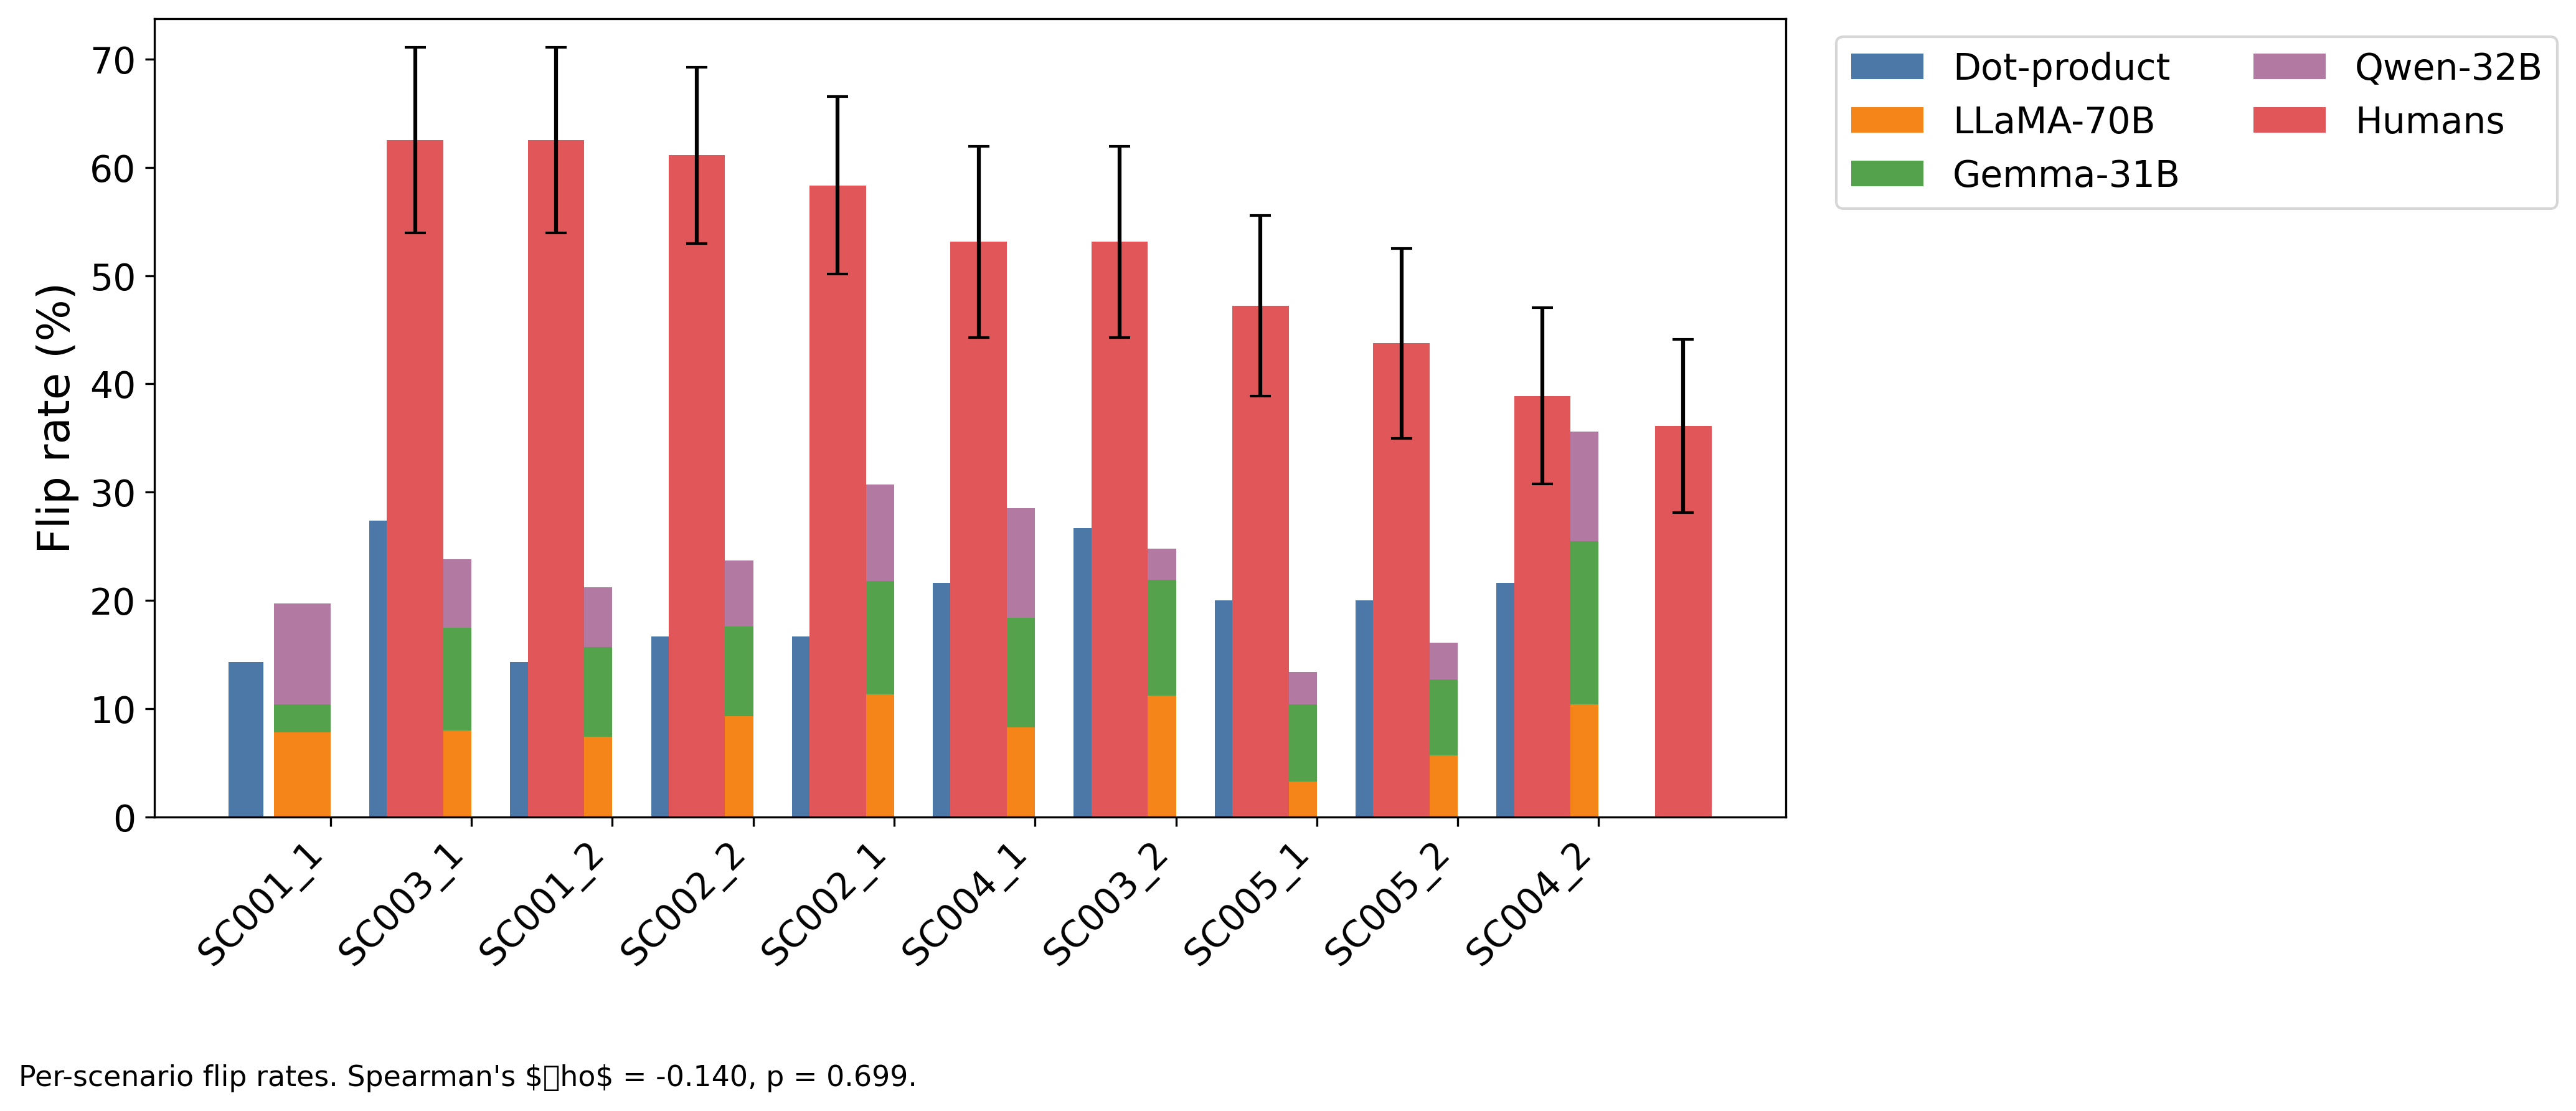
\includegraphics[width=0.95\linewidth]{per_scenario_flip_rates.png}
\caption{Per-scenario flip rates across systems. The dot-product baseline (DP) is uniformly above all LLMs; humans (under the cross-sibling proxy) are uniformly above DP.}
\label{fig:per_scenario}
\end{figure}

\section{Cohen's Kappa Between Humans and LLMs}
\label{app:kappa}

Per-participant Cohen's $\kappa$ between human cross-sibling flip indicators and LLM flip indicators on the same modifier IDs is approximately zero for all three model comparisons (dotProduct, Gemma 4, Llama 8B). This is consistent with our methodological note in \S\ref{sec:method}: the human metric is between-sibling (with scenario-level noise) while the LLM metric is within-profile, so direct binary alignment is not expected. A pre-registered between-subjects re-analysis with PVQ-profile matching is the planned follow-up.

\begin{figure}[H]
\centering
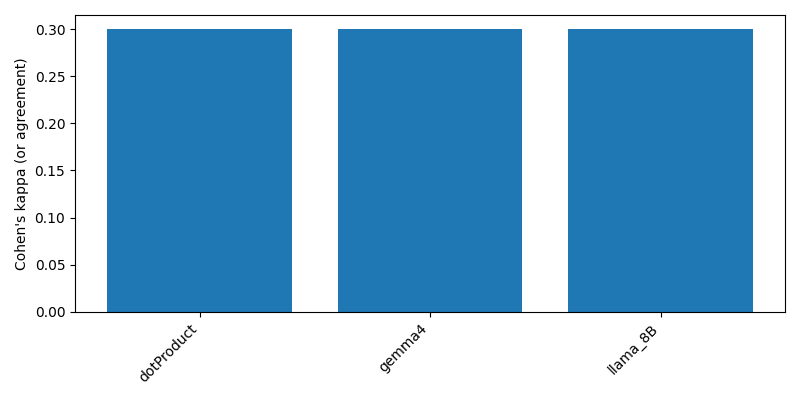
\includegraphics[width=0.7\linewidth]{kappa_bar.png}
\caption{Cohen's $\kappa$ per model (current proxy alignment; expected to rise under profile-matched analysis).}
\label{fig:kappa}
\end{figure}

\section{Qualitative Examples}
\label{app:qualitative}

\paragraph{Example 1 (Llama 3.3 70B, authority\_signal, $A_0 \to A_1$).}
Profile: high in \emph{Hedonism, Power, Conformity, Tradition, Universalism} (5 HIGH). Scenario SC003\_1 (team vs.\ individual recognition). Baseline decision: $A_0$ (recognize the entire team). Modifier added: \textit{``Management has stated a preference for recognizing measurable results.''} Modified decision: $A_1$ (recognize the top individual contributor). Model rationale: \textit{``Recognizing the top individual contributor aligns with my desire for power by identifying a clear leader, and also conforms to management's preference for measurable results.''}

\paragraph{Example 2 (Llama 3.3 70B, authority\_signal, $A_0 \to A_1$).}
Profile: 6 HIGH including \emph{Conformity, Benevolence}. Scenario SC004\_2 (festival vs.\ maintenance). Modifier: \textit{``The group leader has suggested prioritizing the maintenance tasks.''} Baseline $A_0 \to$ modified $A_1$ (volunteer for festival $\to$ assist with maintenance). Rationale invokes both stability values and explicit conformity to leader.

\end{document}
